\documentclass[ignorenonframetext,]{beamer}
\setbeamertemplate{caption}[numbered]
\setbeamertemplate{caption label separator}{: }
\setbeamercolor{caption name}{fg=normal text.fg}
\beamertemplatenavigationsymbolsempty
\usepackage{lmodern}
\usepackage{amssymb,amsmath}
\usepackage{ifxetex,ifluatex}
\usepackage{fixltx2e} % provides \textsubscript
\ifnum 0\ifxetex 1\fi\ifluatex 1\fi=0 % if pdftex
  \usepackage[T1]{fontenc}
  \usepackage[utf8]{inputenc}
\else % if luatex or xelatex
  \ifxetex
    \usepackage{mathspec}
  \else
    \usepackage{fontspec}
  \fi
  \defaultfontfeatures{Ligatures=TeX,Scale=MatchLowercase}
\fi
% use upquote if available, for straight quotes in verbatim environments
\IfFileExists{upquote.sty}{\usepackage{upquote}}{}
% use microtype if available
\IfFileExists{microtype.sty}{%
\usepackage{microtype}
\UseMicrotypeSet[protrusion]{basicmath} % disable protrusion for tt fonts
}{}
\newif\ifbibliography
\hypersetup{
            pdftitle={Class 7: An introduction to Bayesian Statistics},
            pdfauthor={Andrew Parnell},
            pdfborder={0 0 0},
            breaklinks=true}
\urlstyle{same}  % don't use monospace font for urls
\usepackage{color}
\usepackage{fancyvrb}
\newcommand{\VerbBar}{|}
\newcommand{\VERB}{\Verb[commandchars=\\\{\}]}
\DefineVerbatimEnvironment{Highlighting}{Verbatim}{commandchars=\\\{\}}
% Add ',fontsize=\small' for more characters per line
\usepackage{framed}
\definecolor{shadecolor}{RGB}{248,248,248}
\newenvironment{Shaded}{\begin{snugshade}}{\end{snugshade}}
\newcommand{\KeywordTok}[1]{\textcolor[rgb]{0.13,0.29,0.53}{\textbf{#1}}}
\newcommand{\DataTypeTok}[1]{\textcolor[rgb]{0.13,0.29,0.53}{#1}}
\newcommand{\DecValTok}[1]{\textcolor[rgb]{0.00,0.00,0.81}{#1}}
\newcommand{\BaseNTok}[1]{\textcolor[rgb]{0.00,0.00,0.81}{#1}}
\newcommand{\FloatTok}[1]{\textcolor[rgb]{0.00,0.00,0.81}{#1}}
\newcommand{\ConstantTok}[1]{\textcolor[rgb]{0.00,0.00,0.00}{#1}}
\newcommand{\CharTok}[1]{\textcolor[rgb]{0.31,0.60,0.02}{#1}}
\newcommand{\SpecialCharTok}[1]{\textcolor[rgb]{0.00,0.00,0.00}{#1}}
\newcommand{\StringTok}[1]{\textcolor[rgb]{0.31,0.60,0.02}{#1}}
\newcommand{\VerbatimStringTok}[1]{\textcolor[rgb]{0.31,0.60,0.02}{#1}}
\newcommand{\SpecialStringTok}[1]{\textcolor[rgb]{0.31,0.60,0.02}{#1}}
\newcommand{\ImportTok}[1]{#1}
\newcommand{\CommentTok}[1]{\textcolor[rgb]{0.56,0.35,0.01}{\textit{#1}}}
\newcommand{\DocumentationTok}[1]{\textcolor[rgb]{0.56,0.35,0.01}{\textbf{\textit{#1}}}}
\newcommand{\AnnotationTok}[1]{\textcolor[rgb]{0.56,0.35,0.01}{\textbf{\textit{#1}}}}
\newcommand{\CommentVarTok}[1]{\textcolor[rgb]{0.56,0.35,0.01}{\textbf{\textit{#1}}}}
\newcommand{\OtherTok}[1]{\textcolor[rgb]{0.56,0.35,0.01}{#1}}
\newcommand{\FunctionTok}[1]{\textcolor[rgb]{0.00,0.00,0.00}{#1}}
\newcommand{\VariableTok}[1]{\textcolor[rgb]{0.00,0.00,0.00}{#1}}
\newcommand{\ControlFlowTok}[1]{\textcolor[rgb]{0.13,0.29,0.53}{\textbf{#1}}}
\newcommand{\OperatorTok}[1]{\textcolor[rgb]{0.81,0.36,0.00}{\textbf{#1}}}
\newcommand{\BuiltInTok}[1]{#1}
\newcommand{\ExtensionTok}[1]{#1}
\newcommand{\PreprocessorTok}[1]{\textcolor[rgb]{0.56,0.35,0.01}{\textit{#1}}}
\newcommand{\AttributeTok}[1]{\textcolor[rgb]{0.77,0.63,0.00}{#1}}
\newcommand{\RegionMarkerTok}[1]{#1}
\newcommand{\InformationTok}[1]{\textcolor[rgb]{0.56,0.35,0.01}{\textbf{\textit{#1}}}}
\newcommand{\WarningTok}[1]{\textcolor[rgb]{0.56,0.35,0.01}{\textbf{\textit{#1}}}}
\newcommand{\AlertTok}[1]{\textcolor[rgb]{0.94,0.16,0.16}{#1}}
\newcommand{\ErrorTok}[1]{\textcolor[rgb]{0.64,0.00,0.00}{\textbf{#1}}}
\newcommand{\NormalTok}[1]{#1}
\usepackage{graphicx,grffile}
\makeatletter
\def\maxwidth{\ifdim\Gin@nat@width>\linewidth\linewidth\else\Gin@nat@width\fi}
\def\maxheight{\ifdim\Gin@nat@height>\textheight0.8\textheight\else\Gin@nat@height\fi}
\makeatother
% Scale images if necessary, so that they will not overflow the page
% margins by default, and it is still possible to overwrite the defaults
% using explicit options in \includegraphics[width, height, ...]{}
\setkeys{Gin}{width=\maxwidth,height=\maxheight,keepaspectratio}

% Prevent slide breaks in the middle of a paragraph:
\widowpenalties 1 10000
\raggedbottom

\AtBeginPart{
  \let\insertpartnumber\relax
  \let\partname\relax
  \frame{\partpage}
}
\AtBeginSection{
  \ifbibliography
  \else
    \let\insertsectionnumber\relax
    \let\sectionname\relax
    \frame{\sectionpage}
  \fi
}
\AtBeginSubsection{
  \let\insertsubsectionnumber\relax
  \let\subsectionname\relax
  \frame{\subsectionpage}
}

\setlength{\parindent}{0pt}
\setlength{\parskip}{6pt plus 2pt minus 1pt}
\setlength{\emergencystretch}{3em}  % prevent overfull lines
\providecommand{\tightlist}{%
  \setlength{\itemsep}{0pt}\setlength{\parskip}{0pt}}
\setcounter{secnumdepth}{0}
\usepackage{graphicx}
\usepackage{amsmath,amsfonts,amssymb,amsthm,amscd, mathrsfs}
\setbeamertemplate{navigation symbols}{} %%removes bottom line
\setbeamertemplate{footline}[frame number]

\title{Class 7: An introduction to Bayesian Statistics}
\author{Andrew Parnell\newline \texttt{andrew.parnell@mu.ie}
\newline \vspace{1cm} \newline 
\includegraphics[width=5cm]{MU_logo.jpg}}
\date{}

\begin{document}
\frame{\titlepage}

\begin{frame}{Learning outcomes}

\begin{itemize}
\tightlist
\item
  Understand the terms prior, likelihood and posterior
\item
  Know what a posterior probability distribution is, and why we take
  samples from it
\item
  Know how to formulate a linear regression model in a Bayesian format
\item
  Be able to suggest appropriate prior distributions for different
  situations
\end{itemize}

\end{frame}

\begin{frame}{Who was Bayes?}

\emph{An essay towards solving a problem on the doctrine of chances}
(1763)

\[P(A|B) = \frac{P(B|A) P(A)}{P(B)}\]

\begin{center}
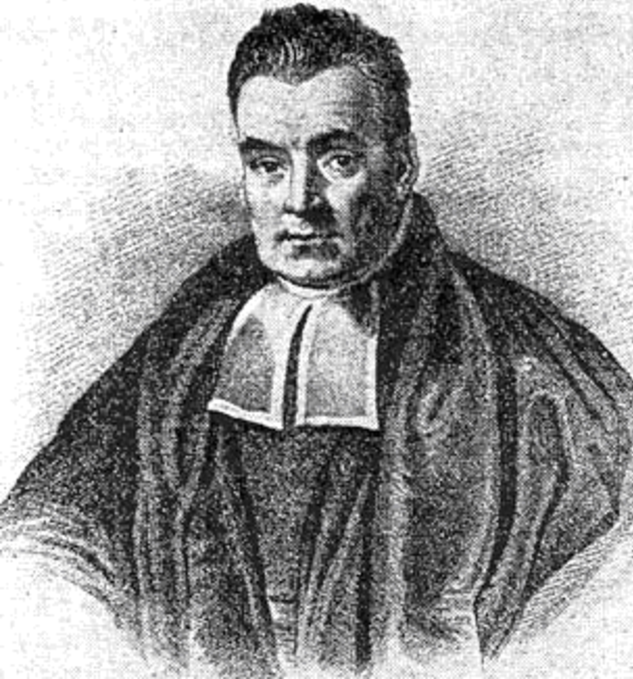
\includegraphics[width=4cm]{Thomas_Bayes.pdf}
\end{center}

\end{frame}

\begin{frame}{What is Bayesian statistics?}

\begin{itemize}
\tightlist
\item
  Bayesian statistics is based on an interpretation of Bayes' theorem
\item
  All quantities are divided up into \emph{data} (i.e.~things which have
  been observed) and \emph{parameters} (i.e.~things which haven't been
  observed)
\item
  We use Bayes' interpretation of the theorem to get the \emph{posterior
  probability distribution}, the probability of the unobserved given the
  observed
\item
  Used now in almost all areas of statistical application (finance,
  medicine, environmetrics, gambling, etc, etc)
\end{itemize}

\end{frame}

\begin{frame}{Why Bayes?}

The Bayesian approach has numerous advantages:

\begin{itemize}
\tightlist
\item
  It's easier to build complex models and to analyse the parameters you
  want directly
\item
  We automatically obtain the best parameter estimates and their
  uncertainty from the posterior samples
\item
  It allows us to get away from (terrible) null hypothesis testing and
  \(p\)-values
\end{itemize}

\end{frame}

\begin{frame}{Bayes theorem in english}

Bayes' theorem can be written in words as:

\[\mbox{posterior is proportional to likelihood times prior}\] \ldots{}
or \ldots{}
\[\mbox{posterior} \propto \mbox{likelihood} \times \mbox{prior}\]

Each of the three terms \emph{posterior}, \emph{likelihood}, and
\emph{prior} are \emph{probability distributions} (pdfs).

In a Bayesian model, every item of interest is either data (which we
will write as \(x\)) or parameters (which we will write as \(\theta\)).
Often the parameters are divided up into those of interest, and other
\emph{nuisance parameters}

\end{frame}

\begin{frame}{Bayes theorem in maths}

Bayes' equation is usually written mathematically as:
\[p(\theta|x) \propto p(x|\theta) \times p(\theta)\] or, more fully:
\[p(\theta|x) = \frac{p(x|\theta) \times p(\theta)}{p(x)}\]

\begin{itemize}
\tightlist
\item
  The \emph{posterior} is the probability of the parameters given the
  data
\item
  The \emph{likelihood} is the probability of observing the data given
  the parameters (unknowns)
\item
  The \emph{prior} represents external knowledge about the parameters
\end{itemize}

\end{frame}

\begin{frame}{A very simple linear regression example}

Suppose you had some data that looked like this:
\includegraphics{class_7_intro_bayes_files/figure-beamer/unnamed-chunk-1-1.pdf}

\end{frame}

\begin{frame}[fragile]{What you are used to doing}

\tiny

\begin{Shaded}
\begin{Highlighting}[]
\NormalTok{mod_lm =}\StringTok{ }\KeywordTok{lm}\NormalTok{(y }\OperatorTok{~}\StringTok{ }\NormalTok{x_centered, }\DataTypeTok{data =}\NormalTok{ dat)}
\KeywordTok{summary}\NormalTok{(mod_lm)}
\end{Highlighting}
\end{Shaded}

\begin{verbatim}
## 
## Call:
## lm(formula = y ~ x_centered, data = dat)
## 
## Residuals:
##     Min      1Q  Median      3Q     Max 
## -4.4351 -0.3705  0.1615  0.5761  2.3302 
## 
## Coefficients:
##             Estimate Std. Error t value Pr(>|t|)    
## (Intercept) 9.737358   0.027858 349.540  < 2e-16 ***
## x_centered  0.022555   0.002866   7.869 8.84e-15 ***
## ---
## Signif. codes:  0 '***' 0.001 '**' 0.01 '*' 0.05 '.' 0.1 ' ' 1
## 
## Residual standard error: 0.9066 on 1057 degrees of freedom
## Multiple R-squared:  0.05533,    Adjusted R-squared:  0.05444 
## F-statistic: 61.91 on 1 and 1057 DF,  p-value: 8.836e-15
\end{verbatim}

\normalsize

\end{frame}

\begin{frame}[fragile]{What you will now get instead}

\tiny

\begin{Shaded}
\begin{Highlighting}[]
\KeywordTok{library}\NormalTok{(rstanarm)}
\NormalTok{mod_stan =}\StringTok{ }\KeywordTok{stan_lm}\NormalTok{(y }\OperatorTok{~}\StringTok{ }\NormalTok{x_centered, }\DataTypeTok{data =}\NormalTok{ dat,}
               \DataTypeTok{prior =} \KeywordTok{R2}\NormalTok{(}\DataTypeTok{location =} \FloatTok{0.5}\NormalTok{, }\StringTok{'mean'}\NormalTok{))}
\end{Highlighting}
\end{Shaded}

\begin{Shaded}
\begin{Highlighting}[]
\NormalTok{mod_stan}
\end{Highlighting}
\end{Shaded}

\begin{verbatim}
## stan_lm
##  family:       gaussian [identity]
##  formula:      y ~ x_centered
##  observations: 1059
##  predictors:   2
## ------
##               Median MAD_SD
## (Intercept)    9.7    0.0  
## x_centered     0.0    0.0  
## sigma          0.9    0.0  
## log-fit_ratio -0.1    0.0  
## R2             0.1    0.0  
## 
## Sample avg. posterior predictive distribution of y:
##          Median MAD_SD
## mean_PPD 9.7    0.0   
## 
## ------
## For info on the priors used see help('prior_summary.stanreg').
\end{verbatim}

\end{frame}

\begin{frame}[fragile]{And yet more detail}

\tiny

\begin{Shaded}
\begin{Highlighting}[]
\KeywordTok{summary}\NormalTok{(mod_stan)}
\end{Highlighting}
\end{Shaded}

\begin{verbatim}
## 
## Model Info:
## 
##  function:     stan_lm
##  family:       gaussian [identity]
##  formula:      y ~ x_centered
##  algorithm:    sampling
##  priors:       see help('prior_summary')
##  sample:       4000 (posterior sample size)
##  observations: 1059
##  predictors:   2
## 
## Estimates:
##                 mean    sd      2.5%    25%     50%     75%     97.5%
## (Intercept)       9.7     0.0     9.7     9.7     9.7     9.8     9.8
## x_centered        0.0     0.0     0.0     0.0     0.0     0.0     0.0
## sigma             0.9     0.0     0.9     0.9     0.9     0.9     0.9
## log-fit_ratio    -0.1     0.0    -0.2    -0.2    -0.1    -0.1    -0.1
## R2                0.1     0.0     0.0     0.1     0.1     0.1     0.1
## mean_PPD          9.7     0.0     9.7     9.7     9.7     9.8     9.8
## log-posterior -1401.1     1.2 -1404.3 -1401.7 -1400.8 -1400.3 -1399.8
## 
## Diagnostics:
##               mcse Rhat n_eff
## (Intercept)   0.0  1.0  1951 
## x_centered    0.0  1.0  1504 
## sigma         0.0  1.0  1988 
## log-fit_ratio 0.0  1.0  1230 
## R2            0.0  1.0  1308 
## mean_PPD      0.0  1.0  2837 
## log-posterior 0.0  1.0  1611 
## 
## For each parameter, mcse is Monte Carlo standard error, n_eff is a crude measure of effective sample size, and Rhat is the potential scale reduction factor on split chains (at convergence Rhat=1).
\end{verbatim}

\end{frame}

\begin{frame}[fragile]{And in a slightly neater format}

\begin{Shaded}
\begin{Highlighting}[]
\KeywordTok{posterior_interval}\NormalTok{(mod_stan)}
\end{Highlighting}
\end{Shaded}

\begin{verbatim}
##                        5%         95%
## (Intercept)    9.69121526  9.78320303
## x_centered     0.01797973  0.02740173
## sigma          0.87416903  0.93916298
## log-fit_ratio -0.19844181 -0.10302552
## R2             0.04474526  0.11742512
\end{verbatim}

\end{frame}

\begin{frame}[fragile]{Using prior information}

\begin{itemize}
\tightlist
\item
  The Bayesian model (hidden in \texttt{stan\_lm}) divided up everything
  into \emph{parameters} (the intercept, slope and residual standard
  deviation), and data (the height and log(earnings) values)
\item
  The software in the background created a posterior probability
  distribution of the parameters given the data
\item
  The model I fitted used vague \emph{prior information}. However, if we
  had done a previous experiment that suggested that the mean \(R^2\)
  value should be around 0.01 we can put that into the model
\end{itemize}

\end{frame}

\begin{frame}[fragile]{With prior information}

\begin{Shaded}
\begin{Highlighting}[]
\NormalTok{mod_stan_}\DecValTok{2}\NormalTok{ =}\StringTok{ }\KeywordTok{stan_lm}\NormalTok{(y }\OperatorTok{~}\StringTok{ }\NormalTok{x_centered, }\DataTypeTok{data =}\NormalTok{ dat,}
               \DataTypeTok{prior =} \KeywordTok{R2}\NormalTok{(}\DataTypeTok{location =} \FloatTok{0.01}\NormalTok{, }\StringTok{'mean'}\NormalTok{))}
\end{Highlighting}
\end{Shaded}

\begin{Shaded}
\begin{Highlighting}[]
\KeywordTok{posterior_interval}\NormalTok{(mod_stan_}\DecValTok{2}\NormalTok{)}
\end{Highlighting}
\end{Shaded}

\begin{verbatim}
##                        5%         95%
## (Intercept)    9.68932534  9.78496979
## x_centered     0.01573809  0.02434343
## sigma          0.87888666  0.94311176
## log-fit_ratio -0.17574214 -0.08593775
## R2             0.03339951  0.08814507
\end{verbatim}

\end{frame}

\begin{frame}[fragile]{What's really happening in the background}

\begin{itemize}
\tightlist
\item
  \texttt{rstanarm} uses \texttt{rstan} to produce these posterior
  distributions
\item
  The idea of \texttt{rstanarm} is to make it easy to switch from
  traditional modelling packages (e.g. \texttt{lme4}) to Bayesian ones
  without too many code changes
\item
  However it does have some very odd ideas about how people include
  prior information, and is somewhat overly mathematical in its
  documentation
\end{itemize}

\end{frame}

\begin{frame}[fragile]{The real \texttt{stan} code}

\scriptsize

\begin{Shaded}
\begin{Highlighting}[]
\NormalTok{stan_code =}\StringTok{ '}
\StringTok{data \{}
\StringTok{  int N;}
\StringTok{  vector[N] x;}
\StringTok{  vector[N] y;}
\StringTok{\}}
\StringTok{parameters \{}
\StringTok{  real intercept;}
\StringTok{  real slope;}
\StringTok{  real<lower=0> residual_sd;}
\StringTok{\} }
\StringTok{model \{}
\StringTok{  // Likelihood}
\StringTok{  y ~ normal(intercept + slope * x, residual_sd);}
\StringTok{  // Priors}
\StringTok{  intercept ~ normal(0, 100);}
\StringTok{  slope ~ normal(0, 100);}
\StringTok{  residual_sd ~ uniform(0, 100);}
\StringTok{\}}
\StringTok{'}
\end{Highlighting}
\end{Shaded}

\end{frame}

\begin{frame}[fragile]{Understanding the different parts of a Bayesian
model}

\begin{itemize}
\tightlist
\item
  The likelihood is the probability of observing the data given the
  parameters. It represents the \emph{data generating process}
\item
  The prior is the probability distribution of the parameters
  independent from the current data you have been generated. It often
  requires care (and philosophy) to choose. More on this later
\item
  The posterior is the probability distribution of the parameters given
  the data. It is always the target of our inference
\item
  The two software packages we will explore (\texttt{rstanarm} and
  \texttt{rstan}), create the posterior distribution for us
\end{itemize}

\end{frame}

\begin{frame}{Lots of probability distributions}

Almost always, the likelihood and prior can be picked from the standard
probability distributions:

\tiny

\begin{tabular}{p{3cm}lp{4cm}}
\hline
Distribution & Range of data & Useful for \\
\hline
Normal, $N(\mu,\sigma^2)$ & $(-\infty,\infty$) & A good default choice \\
Uniform, $U(a,b)$ & $(a,b)$ & Vague priors when we only know the range of the parameter \\
Beta, $Be(\alpha,\beta)$ & $[0,1]$ & Probabilities restriced to be between 0 and 1 \\
t, $t(\mu, \sigma)$ & $(-\infty,\infty$) & Potentially long-tailed or data containing outliers \\
Gamma, $Ga(\alpha,\beta)$ & $(0,\infty)$ & Continuous data with a lower bound of zero \\
Multivariate Normal, $MVN(\mu,\Sigma)$ & $(-\infty,\infty$) & Multivariate unbounded data with correlation between parameters/observations \\
\hline
\end{tabular}

\normalsize
The more probability distributions you know the better you will be at
Bayes!

\end{frame}

\begin{frame}{Practical differences between frequentist statistics and
Bayes}

\begin{itemize}
\tightlist
\item
  In frequentist statistics you tend to get a single best estimate of a
  parameter and a standard error, often assumed normally distributed,
  and a p-value
\item
  In Bayesian statistics you get a large set of samples of the parameter
  values which match the data best. You get to choose what you do with
  these
\item
  In frequentist statistics if the p-value is less than 0.05 you win. If
  not you cry and try a different model
\item
  In Bayesian statistics you try to quantify the size of an effect from
  the posterior distribution, or find a particular posterior
  probability, e.g.~P(slope \textgreater{} 0 given the data).
\end{itemize}

\end{frame}

\begin{frame}{Choosing a likelihood and a prior}

\begin{itemize}
\tightlist
\item
  The key to choosing a likelihood is to pick a probability distribution
  which matches your data, e.g.~if it's a continuous measurement and is
  unbounded then a normal distribution. If it's count data bounded above
  and below then a Binomial might be appropriate
\item
  The key to choosing a prior distribution is to choose values which you
  believe represent the reasonable range that the parameter can take, or
  come from a related study in the literature
\item
  Again, use an \emph{informative prior} if possible
\end{itemize}

Note: the shape of the distribution of the response variable is usually
completely unimportant when choosing the likelihood!

\end{frame}

\begin{frame}[fragile]{\texttt{rstan} vs \texttt{rstanarm}}

We will be using two different software tools to calculate posterior
distributions. These represent the state of the art for user-friendly,
research quality Bayesian statistics.

\begin{itemize}
\tightlist
\item
  \texttt{rstan} positives: very flexible, uses sensible distribution
  names, everything is declared, lots of documentation support, written
  by people at the top of the field
\item
  \texttt{rstan} negatives: cannot have discrete parameters, some odd
  declaration choices, slower to run code, code tends to be longer
\item
  \texttt{rstanarm} positives: very quick for simple models, code looks
  very similar to \texttt{lme4}, no declarations required
\item
  \texttt{rstanarm} negatives: confusing prior distributions, not as
  well documented, not as much flexibility in model choice
\end{itemize}

\end{frame}

\begin{frame}[fragile]{Calculating the posterior vs sampling from it}

\begin{itemize}
\item
  There are two ways to get at a posterior:

  \begin{enumerate}
  \def\labelenumi{\arabic{enumi}.}
  \tightlist
  \item
    Calculate it directly using hard maths
  \item
    Use a simulation method
  \end{enumerate}
\item
  Number 1 is impractical once you move beyond a few parameters, so
  number 2 is used by almost everybody
\item
  This means that we create \emph{samples} from the posterior
  distribution. Here are three samples from the earnings example:
\end{itemize}

\tiny

\begin{verbatim}
##   (Intercept) x_centered     sigma log-fit_ratio         R2
## 1    9.739641 0.02348415 0.8780837    -0.1895515 0.08763874
## 2    9.735334 0.02372870 0.8805866    -0.1876774 0.08913875
## 3    9.765153 0.02462514 0.9254446    -0.1363645 0.08663758
\end{verbatim}

\normalsize

\begin{itemize}
\tightlist
\item
  We often create thousands of posterior samples to represent the
  posterior distribution
\end{itemize}

\end{frame}

\begin{frame}{Things you can do with posterior samples}

\begin{itemize}
\tightlist
\item
  Create histograms or density plots:
\item
  Individual summaries such as means, standard deviations, and quantiles
  (e.g.~95\% confidence intervals)
\item
  Joint summaries such as scatter plots or correlations
\item
  Transformations such as logs/exponents, squares/square roots, etc
\end{itemize}

The posterior distribution will usually be stored in a matrix where each
row is a sample, and each column is a different parameter. Having the
posterior distribution enables you to get at exactly the quantities you
are interested in

\end{frame}

\begin{frame}{Summary so far: for and against Bayes}

For:

\begin{itemize}
\tightlist
\item
  A Bayesian model can be simply displayed as a likelihood and a prior.
  Everything is explicit
\item
  Stan finds the posterior distribution for us so we don't need to do
  any maths
\item
  We can get exactly the quantity we are interested in, the probability
  distribution of our unknowns given our knowns
\end{itemize}

Against:

\begin{itemize}
\tightlist
\item
  It can be hard to create a prior distribution (and a likelihood)
\item
  Not having p-values can make papers harder to publish (but this is
  changing)
\end{itemize}

\end{frame}

\begin{frame}{Checking assumptions (e.g.~residuals)}

\begin{itemize}
\tightlist
\item
  Sometimes people, because Bayesian modelling seems much richer and
  incorporates more information, think that their model is perfect
\item
  In reality we need to check our assumptions. This may include:
\end{itemize}

\begin{enumerate}
\def\labelenumi{\arabic{enumi}.}
\tightlist
\item
  Checking residuals in a linear regression model
\item
  Checking whether the parameter values actually match the data
\item
  Seeing whether a simpler or richer model might fit the data better
\end{enumerate}

Some of this we will cover in later classes, but e.g.~traditional
residual analysis for linear regression is still important here

\end{frame}

\begin{frame}[fragile]{The danger of vague priors}

\begin{itemize}
\tightlist
\item
  Suppose you use the prior distribution
  \texttt{intercept\ \textasciitilde{}\ normal(0,\ 100)} in Stan because
  you had very little information about the intercept. Is this a
  reasonable thing to do? Do you honestly believe that the intercept
  might be as small as -200 or as big as 200?
\item
  If you fit a model and the parameters do not match your views about
  the data, there must be some information you have not encoded in the
  prior, go back and change it!
\item
  In more complex models, you need the prior to constrain some of the
  parameters so that the model will fit. These are known as
  \emph{regularisation} priors
\item
  Use an \emph{informative prior} when you can
\end{itemize}

\end{frame}

\begin{frame}{Replication in Science and the horror of p-values}

\begin{itemize}
\tightlist
\item
  We want our findings to be reproducible. We don't want to publish
  something which is only true for our own data
\item
  Unfortunately p-values do not do this because:
\end{itemize}

\begin{enumerate}
\def\labelenumi{\arabic{enumi}.}
\tightlist
\item
  A p-value is essentially a function of the sample size. If you want a
  smaller p-value simply collect more data
\item
  A p-value tells you nothing about the null hypothesis. It's a
  probability on the data assuming the null hypothesis is true!
\item
  The null hypothesis is never true. It's a straw man that is waiting to
  be knocked down by your data
\end{enumerate}

Bayesian hierarchical modelling is a great way to stop using p-values
and start doing reproducible science

\end{frame}

\begin{frame}{General tips}

\begin{itemize}
\item
  If you have lots of disparate data, try to build one model for all of
  it. You'll be able to \emph{borrow strength} from the data (e.g.~in a
  hierarchical model) and reduce the uncertainty in your parameter
  estimates
\item
  Try your hardest to use informative priors, and always justify the
  values you use (especially when trying to publish). In this course
  we're presenting generic examples so have almost always used vague
  priors
\item
  Check your model. Many of the usual requirements from traditional
  statistics (e.g.~residual checks) are still relevant in the Bayesian
  world. There are some extra Bayesian tricks we can also do; discussed
  in later classes
\end{itemize}

\end{frame}

\begin{frame}[fragile]{Summary}

\begin{itemize}
\item
  Bayesian statistical models involve a \emph{likelihood} and a
  \emph{prior}. These both need to be carefully chosen. From these we
  create a posterior distribution
\item
  The likelihood represents the information about the data generating
  process; the prior information about the unknown parameters
\item
  We usually create and analyse samples from the posterior probability
  distribution of the unknowns (the parameters) given the knowns (the
  data)
\item
  From the posterior distribution we can create means, medians, standard
  deviations, credible intervals, etc, from samples we take using e.g.
  \texttt{rstanarm} or \texttt{rstan}
\end{itemize}

\end{frame}

\end{document}
